\section{Motivation}
\label{sec:motivation}

Real-time control of autonomous vehicles requires the processing of a large amount of sensor data, which is used by the vehicle to determine its position in the world and to calculate its next move.
Examples include data from cameras, LIDAR, radars and ultrasound radars, and possibly information communicated by other vehicles or the road infrastructure.
The perception algorithms that process this data must do so fast enough for the control algorithm to compute the next input within the time constraints imposed by the environment.
These time constraints are variable: for example, relaxed rural driving can accommodate planning actions every tens of milliseconds, while imminent collision avoidance requires planning and actuation on the order of a few milliseconds.
As a result of the variability in the environment, and to guarantee adequate performance in the most demanding conditions, the control and perception systems are over-engineered to operate as if the worst-case conditions always hold. 
This results in unnecessarily high power consumption from the computation platform.
%Note that over the past few decades, the power consumption of processors has increased by more than double, while battery energy density has only improved by about a quarter \cite{Lahiri}. 

The usage of \emph{anytime perception algorithms} allows us to perform a trade-off between the computation time of the algorithms, their power consumption, and the quality of their output.
An anytime algorithm has a pre-defined set of interruption times. 
The earlier the algorithm is interrupted, the less power it consumes, but the worse is the quality of its output in general. 
On the other hand, that quality may be sufficient for the control algorithm to achieve its goal \emph{in the current circumstances}.
For example, in this paper, the control objective is to follow the center of a driving lane, and control performance is measured by the deviation from that center.
At slow speeds, poor quality of position estimate may be tolerated since it won't lead to excessive deviations from the center.
Therefore, the perception algorithm might be interrupted early thus saving on computation power, \emph{provided it gives a good enough estimate of position. }

In \cite{RTSS15} we proposed a way in which a standard perception algorithm can be turned into an anytime algorithm via off-line profiling, and thus can offer a time/power/quality trade-off.
We also designed a model predictive controller than can make use of the trade-off offered by the anytime perception algorithm.
To achieve the time/power/quality trade-off, we produced multiple versions of the perception algorithm.
Broadly speaking, a version that ran for longer produced a higher quality output. 

In this work, we turn our attention to the time/power trade-off \emph{for a fixed quality of output} and how it can be achieved using \emph{platform-level} optimizations.
Even when the output quality is fixed, the computation delay (equivalently, throughput) is known to affect control performance. 
Thus in this paper, we study how platform-level optimizations affect the computation throughout and power, and how to use this trade-off to save computation power without overly degrading throughput.

Note that the study of how computation delay affects control performance, and the design of anytime perception and control algorithms for power saving, are not specific to autonomous vehicles.
Other control systems can benefit from these trade-offs, especially power-limited consumer robots.
In this paper, we illustrate our approach on an autonomous car $1/10^{th}$ the size of a regular car (Fig. \ref{fig:traxxas}), which uses Vanishing Point navigation \cite{VP1}.
\begin{figure}[t]
	\centering
	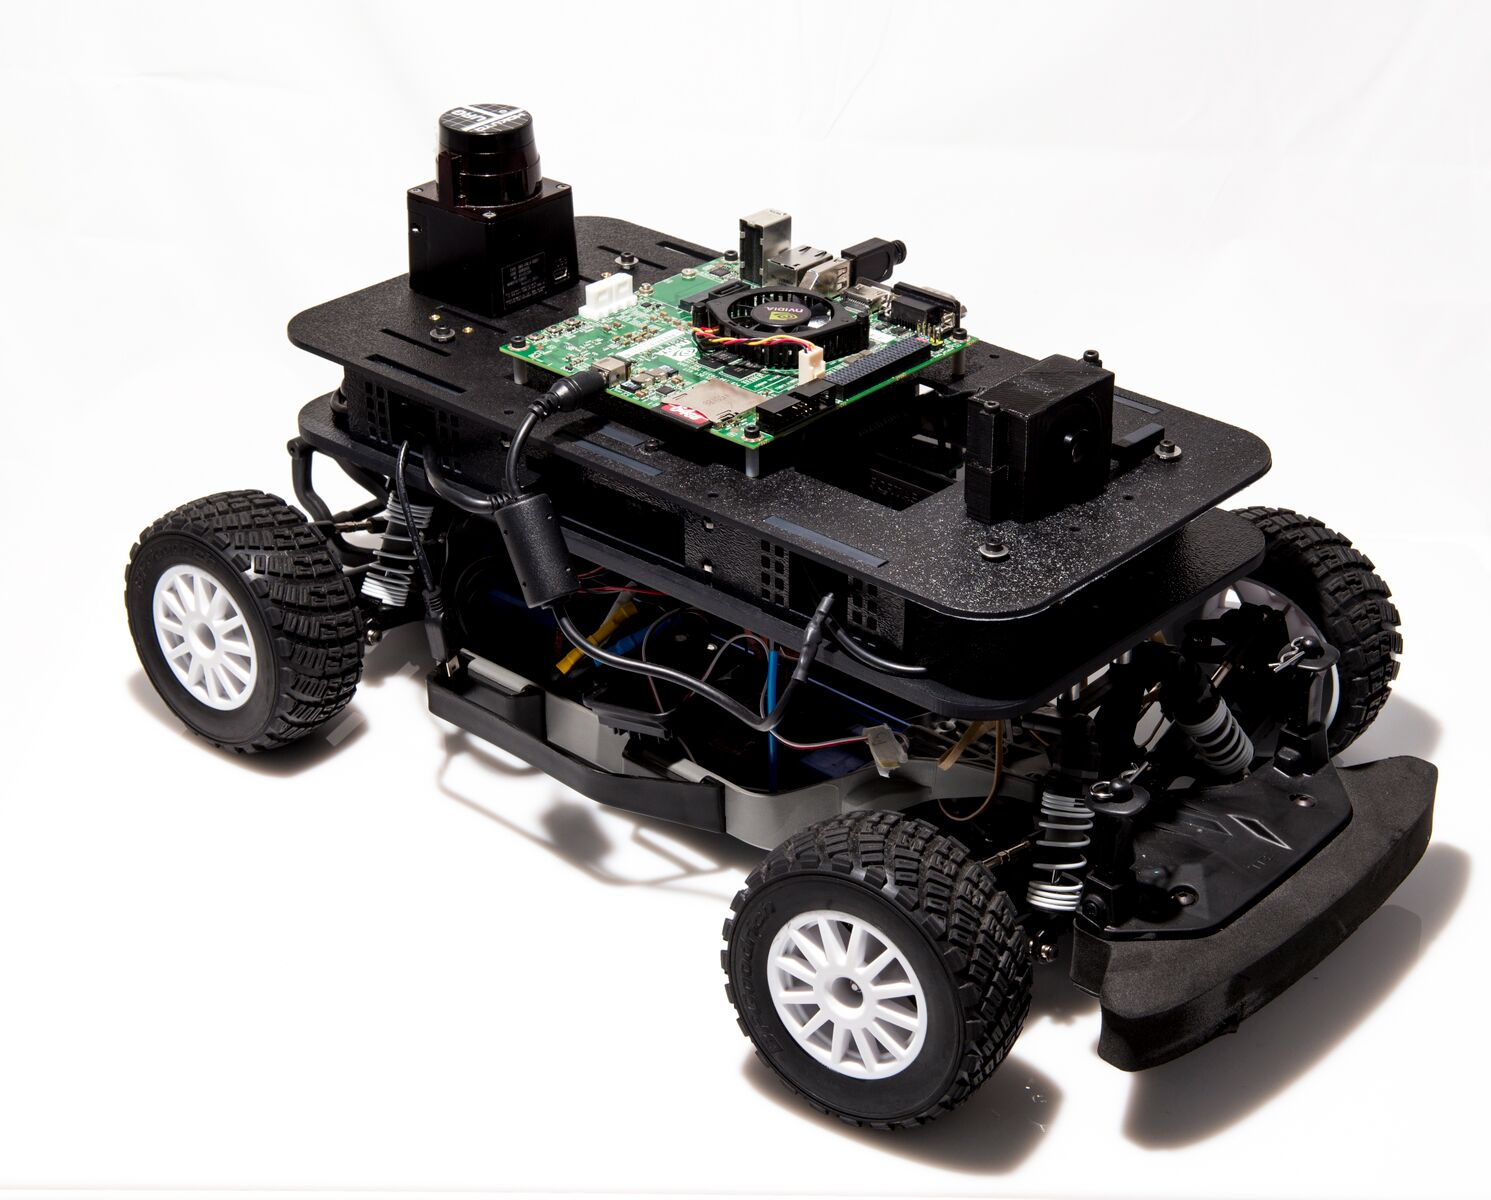
\includegraphics[scale=0.08]{carImages/im4.jpeg}
	\caption{Traxxas autonomous car with camera.}
		\label{fig:traxxas}
\end{figure}  
The setup, including the navigation algorithm, are presented in Section \ref{sec:problemSetup}.
Section \ref{sec:twoStage} describes the offline profiling of Vanishing Point, which gives us Throughput vs Power curves for various processor frequencies and various scheduling of the navigation code on CPU and GPU.
In Section \ref{sec:evaluation} we combine power and throughput into one objective function, and design a supervisor what will determine the frequency and CPU/GPU allocation to maximize the objective.
Section \ref{sec:simResults} presents experimental results that demonstrate the effect of the trade-off on control performance.
%\todo[inline]{give example nb}
%
%
%Traditionally, perception algorithms were designed without consideration for the context in which their outputs will be produced
%Since the ultimaSince the meaning of real-time depends on the context, and 
%
%One impediment to achieving this real-time scalability variability 
%  presents In recent years, autonomous cars have become more and more prolific and increasingly capable \cite{}. For the perception and control software of these systems, there are stringent real-time requirements that have to be met for the safe performance of the system. In order for these requirements to be met, autonomous systems (both their hardware and software) are overengineered, resulting in a power consumption for the computation tasks that is not negligible. Also, while the focus of reducing power consumption in the design of such systems has been mostly on the power consumed by the actuators, computational platforms have been consuming more and more power. 
%It is worth noting that over the past few decades, the power consumption of processors has increased by more than double, while battery energy density has only improved by about a quarter [??Rajkumar??]. 
%
%In this poster, we present a method to obtain more energy efficient computations for the perception and estimation algorithms used in autonomous systems by exploiting hardware and algorithm level knobs. These knobs allow us to leverage a tradeoff between power consumption and a measure of quality of the perception and estimation algorithms. On-going work focuses also on coming up with a supervisory algorithm and control algorithms that are aware of this trade-off and choose an optimal operating point (or knobs settings) such that the performance of the overall closed-loop system is safe as well as energy efficient.
%
%Our method consists of a two-phase approach. The first involves extensively profiling the perception and estimation algorithm offline with all knob settings for timing, quality of output (if available) and power consumption. It also involves developing a control rule which chooses the best operating point for the perception and estimation algorithm while ideally providing mathematical guarantees on the safe performance of the system, e.g. as in \cite{} . The second, online stage, involves picking the best operating mode and control setting and run-time monitoring of the system performance. 
%
%We have developed an $1/10^{th}$ scale autonomous car testbed on which we evaluate our methods. In this particular work, we focus on a vanishing point algorithm based autonomous corridor navigation. We look at the algorithm level knobs, which are scheduling the sequential tasks of the vanishing point based algorithm on either the CPU or GPU; and the hardware level knobs which are frequencies of the CPU and GPU. Scheduling the tasks on different resources along with the different hardware settings result in a wide variety of timing and power distributions obtained.   
